\subsection{Calibrazione}\label{par:fondo1}

\begin{figure}
	\centering
	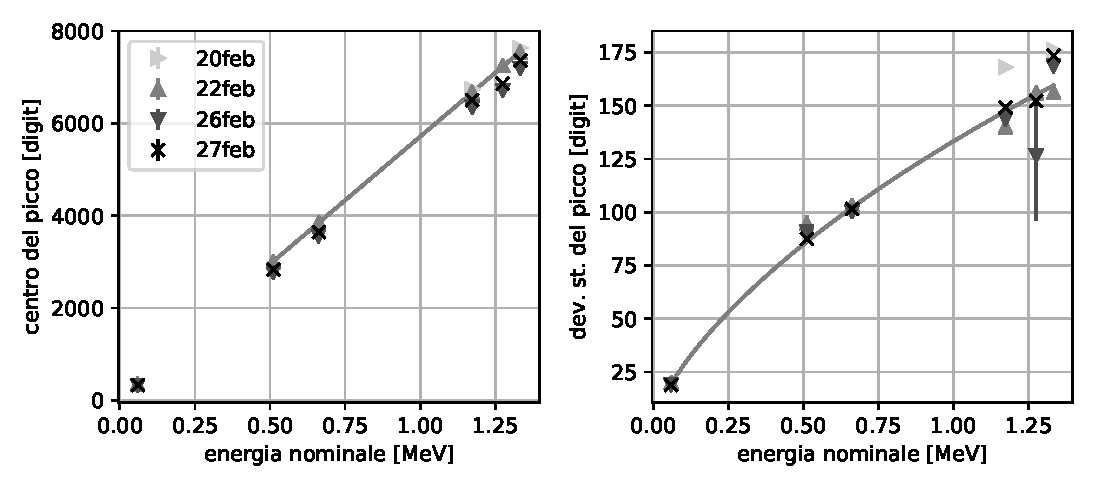
\includegraphics[width=\textwidth]{calibration}
	\caption{\label{fig:calibration}
	Dati per la calibrazione.
	La curva di fit è riportata solo per 22feb.
	Nel fit della scala, il punto a sinistra escluso dal fit è l'americio.}
\end{figure}

\begin{table}
	\centering
	\begin{tabular}{cccc}
		\toprule
		Calibrazione & $m$ [\si{digit\,keV^{-1}}] & $q$ [\si{digit}] & $a$ [\si{digit\,keV^{-1}}] \\
		\midrule
		20feb & \num{5.6(3) } & \num{2(4)e+2} &   \num{4.93(8) } \\
		22feb & \num{5.52(6)} & \num{1.9(7)e+2} & \num{4.39(6) } \\
		26feb & \num{5.39(3)} & \num{11(28)} &    \num{4.52(8) } \\
		27feb & \num{5.49(7)} & \num{2(8)e+1} &   \num{4.49(10)} \\
		\bottomrule
	\end{tabular}
	\caption{\label{tab:calibration}
	Risultato della calibrazione.
	$m$ e $q$ sono i parametri per calibrare la scala di energia,
	$a$ è il parametro per calcolare la risoluzione.}
\end{table}

Per calibrare la scala di energia dell'ADC usiamo le sorgenti ausiliarie.
Poniamo una sorgente alla volta davanti allo spettrometro (con la sorgente principale chiusa e non visibile)
e misuriamo lo spettro.
Fittiamo i fotopicchi con gaussiane più un fondo modellato empiricamente con una retta tagliata alle ordinate negative
(in modo che sia forzatamente positivo).
Da ogni fotopicco otteniamo il centro e la deviazione standard.

\paragraph{Scala dell'energia}

Fittiamo i centri in funzione dell'energia dei fotoni delle sorgenti con una retta $y=mx+q$,
non includendo nel fit l'americio (quello a energia minore)
perché non è nell'intervallo di energie in cui useremo la calibrazione
e il modello lineare non è in accordo statistico con i dati;
per lo stesso motivo moltiplichiamo le incertezze su $m$ e $q$ per il fattore di scala $\sqrt{\chi^2/\mathrm{ndof}}$,
dove il $\chi^2$ è del fit complessivo di tutte le calibrazioni.
Teniamo conto della correlazione dei centri del cobalto.

\paragraph{Risoluzione}

Come modello per la risoluzione in funzione dell'energia usiamo la formula
FONTE CIPPALIPPA
\begin{equation}
	\sigma_E(E) = a \cdot E \cdot \frac{2.27 + 7.28 \cdot E ^ {-0.29} - 2.41 \cdot E ^ {0.21}} {235}
\end{equation}
con $E$ in \si{MeV}, dove fittiamo solo l'ampiezza $a$.
Anche in questo caso moltiplichiamo l'incertezza per il fattore di scala,
ma il fit è separato per ogni calibrazione.
I risultati sono riportati in \autoref{tab:calibration},
i dati in \autoref{fig:calibration}.
